\documentclass[letterpaper, 12pt]{article}

\usepackage{geometry}
 \geometry{
 letterpaper,
 total={170mm,257mm},
 left=20mm,
 top=20mm,
 bottom=20mm
 }
\usepackage{graphicx} % Required for inserting images
\usepackage{authblk}
\usepackage{amssymb}
\usepackage{lipsum}
\usepackage{float}
\usepackage{times}
\usepackage{amsmath}
\usepackage[format=plain,
            labelfont={bf,it},
            textfont=it]{caption}
\captionsetup{justification=raggedright,singlelinecheck=false}
\usepackage{ragged2e}
\usepackage{longtable}
\usepackage{comment}
\usepackage{setspace}
\usepackage{fancyhdr}
\usepackage{titlesec}
\usepackage[hyperindex,breaklinks]{hyperref}
\hypersetup{
    colorlinks=true,
    linkcolor=blue,
    filecolor=magenta,      
    urlcolor=blue,
    pdftitle={Overleaf Example},
    pdfpagemode=FullScreen,
    }
% \usepackage{background} % add COSIG logo to page
\usepackage[T1]{fontenc}
\usepackage{helvet}
\renewcommand{\familydefault}{\sfdefault}
\pagenumbering{gobble}
\usepackage[skip=10pt plus1pt, indent=40pt]{parskip}

\begin{comment}
\backgroundsetup{
   scale=1,
   angle=0,
   opacity=1,
   color=black,
   contents={\begin{tikzpicture}[remember picture, overlay]
      \node at ([xshift=3cm,yshift=1cm] current page.south west)
            {
\includegraphics[width = 5cm]{img/home/241017_final_logo_mockup.png}}; %<- change the name of image
     \end{tikzpicture}}
 }
\end{comment}

\titlespacing*{\section}
{0pt}{1.5ex plus 1ex minus .2ex}{1.3ex plus .2ex}

\renewcommand\Authfont{\fontsize{12}{14.4}\selectfont}
\renewcommand\Affilfont{\fontsize{9}{10.8}\itshape}
 
\begin{document}
\flushleft

\includegraphics[width=0.5\textwidth]{img/home/241017_final_logo_mockup.png}

\section*{Energy-dispersive X-ray spectroscopy}
\textit{Last updated: 6 February 2025}

\href{https://en.wikipedia.org/wiki/Energy-dispersive_X-ray_spectroscopy}{Energy-dispersive X-ray spectroscopy (EDX/EDS/EDAX)} is a popular experimental technique used to characterize the elemental composition of a sample.

EDX typically involves bombarding a sample with high-energy electrons, exactly the kind that are used for scanning electron microscopy (SEM) and transmission electron microscopy (TEM). SEM/TEM instruments are often sold with EDX instruments built-in and EDX instruments are often sold as SEM/TEM accessories.

Atoms contain negatively-charged electrons bound to a positively-charged nucleus at well-defined energy levels. When an atom in a sample is exposed to a beam of high-energy electrons, some of these bound electrons will become excited and leave their energy level or ``shell'', leaving an ``electron hole''. This hole is then filled by another electron dropping from a higher-energy shell, which releases the excess energy required to drop to a lower energy level in the form of an X-ray.

The energy levels electrons occupy are well-defined for each element, meaning that each element will emit X-rays at a series of well-defined characteristic energies. An EDX detector will read the energies of emitted X-rays and construct a spectrum, which can then be analyzed quantitively to determine the elemental composition of a sample.

A typical EDX spectrum will show X-ray energy on the x axis (typically expressed in electron volts, eV) and counts or counts per second (cps) on the y axis (with each ``count'' representing a single detected X-ray emission).

\begin{figure}[h!tbp]
    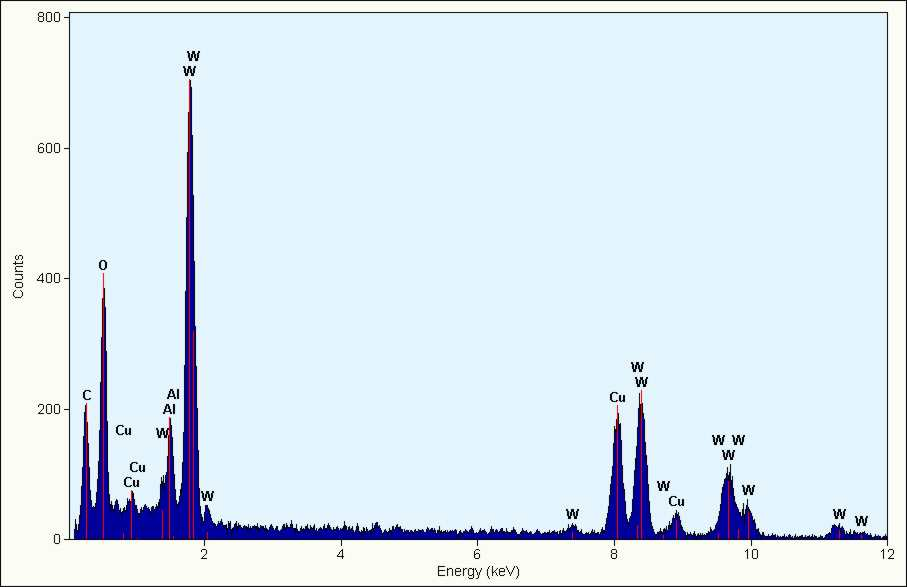
\includegraphics[width=\textwidth]{img/edx/beispiel_EDX.jpg}
    \caption*{ An example EDX spectrum for an aluminum tungsten oxide on a carbon foil supported on a copper grid. Adapted from \href{https://www.microscopy.ethz.ch/xray_spectrum.htm}{material prepared by Dr. Frank Krumeich.}}
\end{figure}

Because the characteristic X-ray emission energies of any element are predictable and well-defined, the height and position of peaks they will produce on an EDX spectrum are also predictable and well-defined. For instance, carbon will only ever produce a single peak at around 277 eV. Silicon will only ever produce two peaks: one around 1.74 keV and another around 1.84 keV. Heavier elements tend to produce more peaks at higher energies.

An EDX spectrum will only ever contain peaks up to the energy of the incident electron beam. For instance, if EDX is performed with an electron beam with an accelerating voltage of 10 kV, no peaks will be observed at energies higher than 10 keV.

The peaks that will be produced by each element can be found in various lookup tables, like \href{https://xdb.lbl.gov/Section1/Periodic_Table/X-ray_Elements.html}{this one from Lawrence Berkeley National Laboratory}. However, the most convenient and comprehensive resource for determining expected peaks is the software \href{https://www.cstl.nist.gov/div837/837.02/epq/dtsa2/index.html}{NIST DTSA-II}. DTSA-II also allows the user to simulate spectra and quantify elemental abundances from real spectra.

\subsection*{Elements not detectable by EDX}

Hydrogen (atomic number 1) and helium (atomic number 2) do not produce characteristic X-rays and are thus not detectable by EDX. Lithium (atomic number 3) and beryllium (atomic number 4) produce characteristic X-rays at such a low energies ($\sim$ 54 and $\sim$ 108 keV, respectively) that most EDX detectors will fail to capture them.

\subsection*{Escape peaks}

Some elements will produce silicon "escape" peaks. These peaks occur with silicon-based detectors (used in the vast majority of EDX instruments) and will appear exactly one Si $K\alpha$ emission energy ($\sim$ 1.7 keV) below prominent peaks produced by an element.

\begin{figure}[h!tbp]
    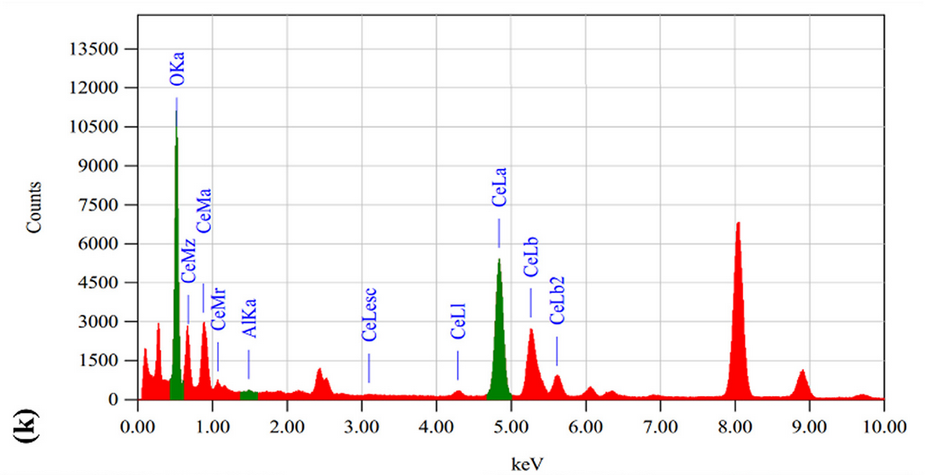
\includegraphics[width=\textwidth]{img/edx/shah_edx.png}
    \caption*{ An example EDX spectrum for a material containing cerium. A faint cerium escape peak is labeled at $\sim$ 3.1 keV. Adapted from Figure 3K of \href{https://doi.org/10.1016/j.ijhydene.2022.12.153}{Shah et al. (2023)}.}
\end{figure}

\subsection*{Mounting grids}

Samples are typically mounted to a metallic grid and/or a thin foil to facilitate handling. The materials used in these grids will often appear in EDX spectra. Grids and foils are most commonly composed of gold, copper, carbon or aluminum.

\subsection*{Zero strobe peak}

Many EDX detectors will insert an artificial peak centered at 0 eV. This peak, called the ``zero strobe'', ``zero strobe peak'' or ``strobe peak'', is used for instrument calibration is often removed before further analysis. If it is left included, it can give the appearance of detection of X-rays with negative energies. While leaving the zero strobe peak included can negatively impact the performance of elemental abundance estimation software, the appearance of a zero strobe peak in a published EDX spectrum is usually no cause for concern.

\begin{figure}[h!tbp]
    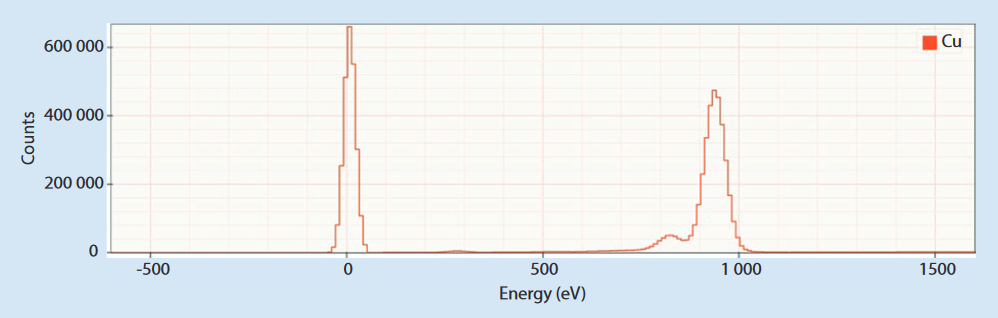
\includegraphics[width=\textwidth]{img/edx/zero_strobe_peak.png}
    \caption*{ An example EDX spectrum for elemental copper showing a zero strobe peak centered around 0 eV. Adapted from Figure 17.7 of \href{https://doi.org/10.1007/978-1-4939-6676-9}{Scanning Electron Microscopy and X-ray Microanalysis}.}
\end{figure}

\pagebreak

\subsection*{Example 1: Problematic EDX spectrum}

\href{https://doi.org/10.1016/j.ijhydene.2024.05.274}{Hussain et al. (2024)} claim to use EDX to characterize the elemental composition of an AgMnTe composite. However, the EDX spectrum they provide in Figure 2C has several issues:

\begin{enumerate}
    \setlength\itemsep{-0.5em}
    \item Tellurium has no peaks between 6 keV and 7 keV.
    \item Manganese has no peak at $\sim$ 6.2 keV.
    \item Manganese has no peak at $\sim$ 5 keV.
\end{enumerate}

\begin{figure}[h!tbp]
    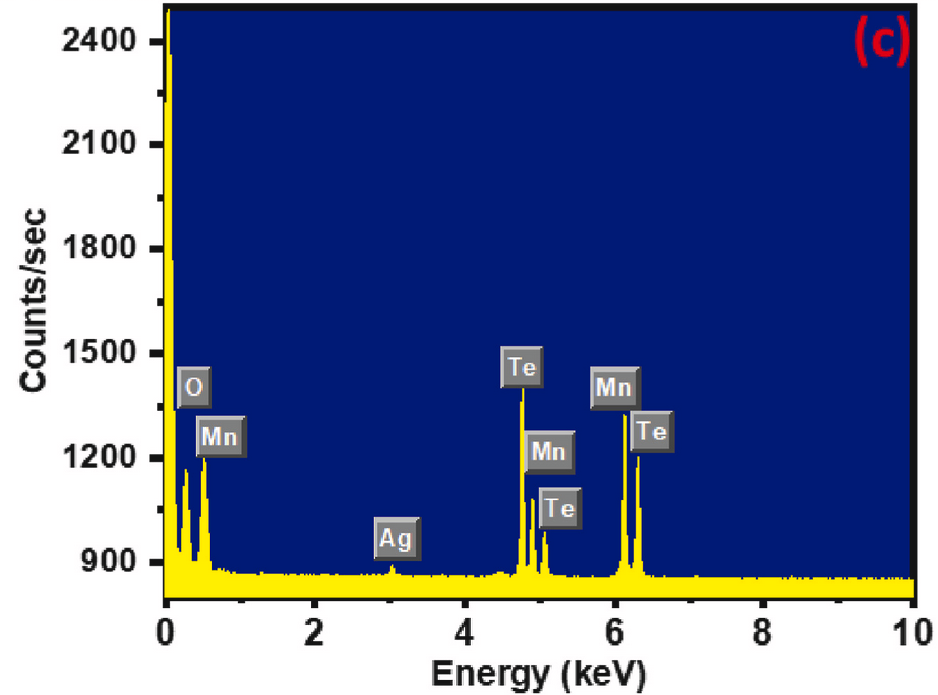
\includegraphics[width=\textwidth]{img/edx/hussain_edx.png}
    \caption*{ A problematic EDX spectrum with several nonsensical peak positions. Adapted from Figure 2C of \href{https://doi.org/10.1016/j.ijhydene.2024.05.274}{Hussain et al. (2024)}.}
\end{figure}

\pagebreak

\subsection*{Example 2: Problematic EDX spectrum}

\href{https://doi.org/10.1007/s10854-022-08265-y}{Alwadai et al. (2022)} claim to use EDX to characterize the elemental composition of polypyrrole, cobalt ferrite, and a poylpyrrole/cobal ferrite composite. However, the spectra they provide have numerous issues:

\begin{enumerate}
    \setlength\itemsep{-0.5em}
    \item Oxygen's sole peak should be at 524.9 eV, but appears in 3A at $\sim$ 0.9 keV.
    \item Oxygen has two peaks in 3B. Oxygen has one peak.
    \item Iron has no peaks between 1 and 4 keV. 3B shows two peaks for iron in this range.
    \item Iron has no peaks > 8 keV, unlike what is shown in 3B.
    \item Cobalt has no peak at $\sim$ 2 keV and no peak at $\sim$ 10 keV, unlike what is shown in 3B.
    \item In increasing order, the lowest energy peaks in 3C should be carbon, nitrogen, oxygen, iron. The order shown in 3C is nitrogen, oxygen, iron, carbon.
    \item Cobalt has no peaks at $\sim$ 5.9 keV. The nearest expected peak is an escape peak at $\sim$ 5.2 keV.
    \item Carbon does not have a peak at $\sim$ 7 keV.
    \item Oxygen does not have a peak at $\sim$ 8 keV.
    \item Hydrogen does not have any peaks, let alone one at $\sim$ 9 keV.
\end{enumerate}

\begin{figure}[h!tbp]
    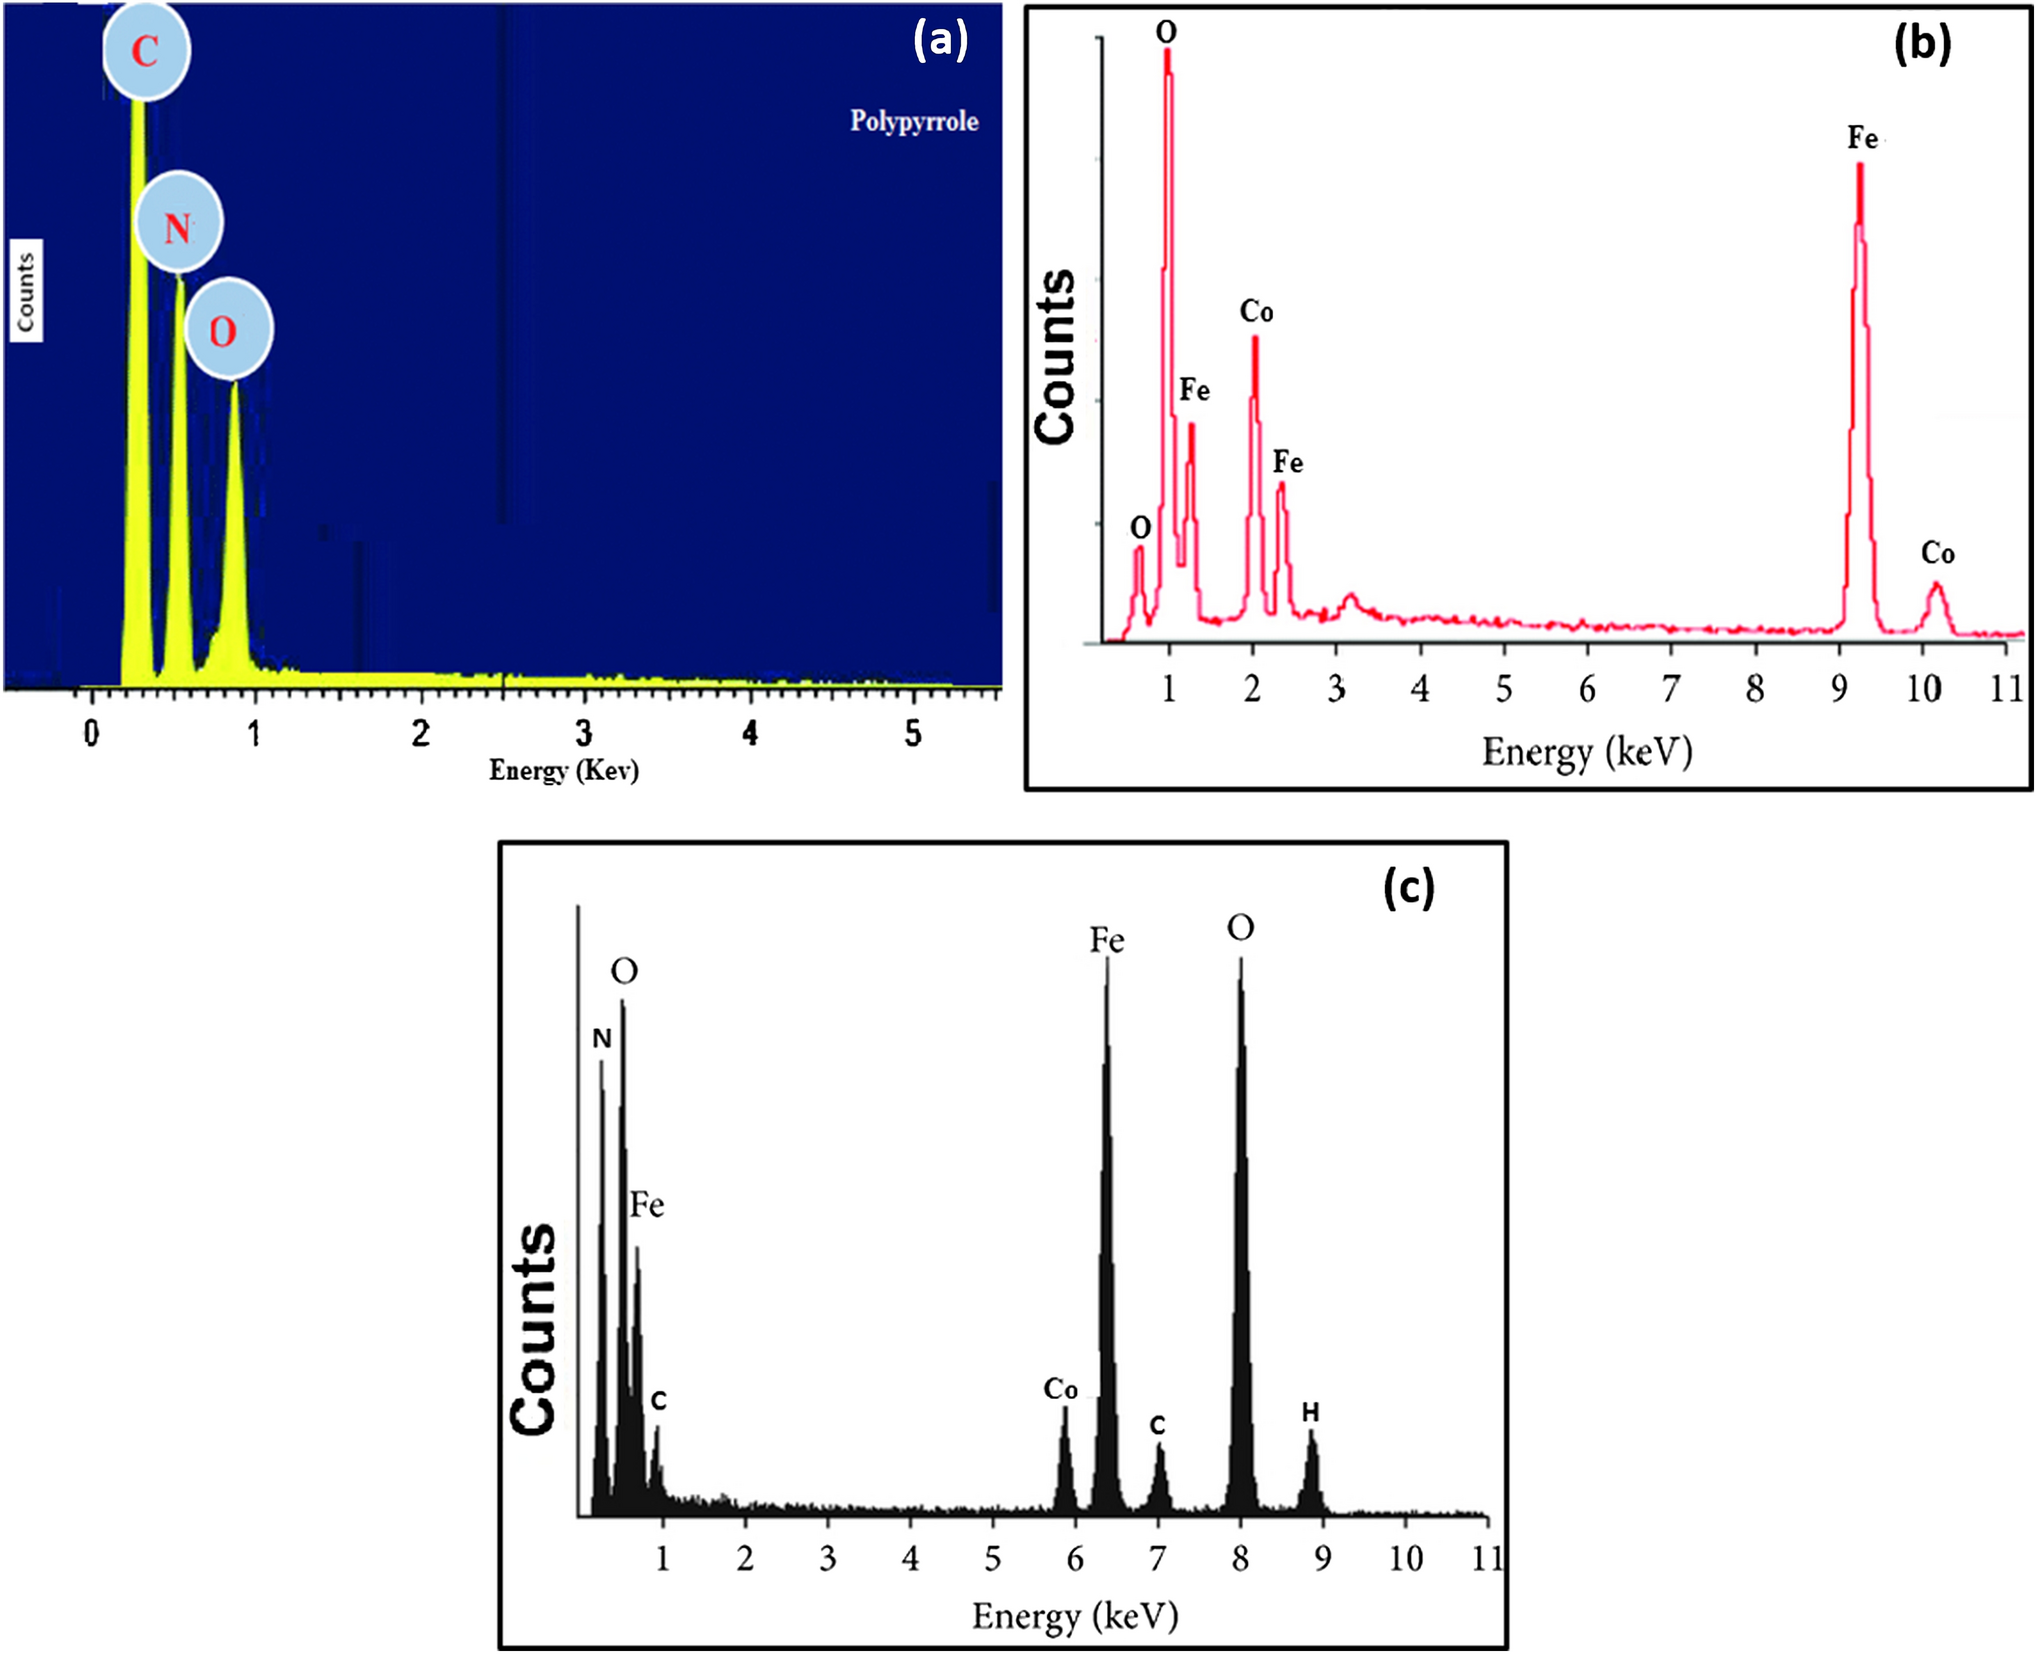
\includegraphics[width=0.8\textwidth]{img/edx/alwadai_edx.png}
    \caption*{Problematic EDX spectra with numerous issues. Adapted from Figure 3 of \href{https://doi.org/10.1007/s10854-022-08265-y}{Alwadai et al. (2022)}.}
\end{figure}

\subsection*{Additional resources}

\begin{itemize}
    \setlength\itemsep{-0.5em}
    \item \href{https://fy.chalmers.se/~f10mh/Halvarsson/EM_intro_course_files/EDX%20intro.pdf}{Lecture notes by Dr. Chris Boothroyd}
    \item \href{https://doi.org/10.1007/978-1-4939-6676-9}{\textit{Scanning Electron Microscopy and X-ray Microanalysis} (textbook)}
\end{itemize}

% \setlength\itemsep{-0.5em}
% for bullet points and numbered lists.

\end{document}